\documentclass{literature}

\title{Exploring the physical properties of high redshift galaxies with KMOS}
\subtitle{First year report}
\author{Owen J. Turner}
\authoremail{turner@roe.ac.uk}
\supervisor{Dr. Michele Cirasuolo}
\supervisoremail{ciras@roe.ac.uk}
\slugheader{First year report}
\slugauthor{Owen J. Turner}
\logo{/Users/owenturner/Documents/PhD/KMOS/Latex/Literature_Review/UoEcrest.pdf}
\graphicspath{{Users/}{owenturner/}{Documents/}{PhD/}{KMOS/}{Latex/}{Literature_Review/}{Figures/}}
\abstract{This is a first year report detailing what I've been up to over my first 9 months as a PhD student and laying out the path that will be taken from here going forwards. }
\setcounter{secnumdepth}{4}


\begin{document}

\coverpage



%%%%%%%%%%%%%%%%%%%%%%%%%%%%%%%%%%%%%%%%%%%%%%%%%%%%%%%%%%%%%%%%%%%%%%%%%%%%%%%%%%%%%%%%%%%%%%%%%%%%%%%%%%%%%%%%%%%%%%


\section{Introduction}\label{sec:Intro}
The physical processes which govern the formation and evolution of high redshift galaxies are representative of a time when the universe was most active. It is the gas within these galaxies which is the driving force behind galaxy evolution, and there are various tools provided by the latest generation of telescope which allow astronomers to explore the properties of this gas. \\ 



Throughout this first year report, I will give a brief overview of how to go between telescope data and the physical properties of a galaxy, indicating the literature surrounding this in section \ref{sec:background}. Section \ref{subsec:current_int} gives an overview of the telescopes 
routinely collecting the spectra of high redshift galaxies, highlighting the wavelength ranges in which their detectors operate and whether 
they have the capacity for integral field spectroscopy. Section \ref{sec:KMOS} focusses specifically on the specifications of KMOS and the key science drivers motivating research with this instrument. 





\section{Background}\label{sec:background}
mini lit review introduction. Set the context 

\citep{Troncoso_2014}, \citep{Maiolino2008}, \citep{Cullen2014}, \citep{Kewley2002}, \citep{Kennicutt_2012}, \citep{Tremonti2004} \citep{Brinchmann2004} \citep{Savaglio2005} \citep{Erb_2006} \citep{Kewley_2008} \citep{ForsterSchreiber2009} \citep{Steidel2014}
Major themes are: 

\begin{itemize}
	\item The need for detailed measurements of high-z galaxies with integral field spectrometers 
	\item a description of available IFS at different portions of the spectrum, kmos optimised for Halpha at z3
	\item Dust
	\item Measurement of abundance 
	\item photoionization models and population synthesis
	\item morphology 
	\item gas dynamics, outflows and the connection between this and evolution 
	\item flux data cubes 
	\item the mass metallicity relation and the fmr 
	\item use of abundance techniques described by cullen 
\end{itemize}

Plots will be: 

\begin{itemize}
	\item peak of SFRd curve 
	\item m-z relation at different epochs 
	\item Attempts to force the strong lines to be equal 
	\item Gradients in physical properties from Troncoso
	\item Some spectra -  
	\item look at all the plots from your other document 
\end{itemize}



M-Z graphs at different redshifts and FMR graphs to illustrate the point. Wanting to confirm the shape of both at redshift 3, or actually looking at the M-Z relation at different points throughout the galaxy - i.e. does the centre of the galaxy follow a different M-Z relation to the outskirts of the galaxy. 

\subsection{Measuring Flux}
Dust extinction, calzetti curves etc. 

 

\subsubsection{Slit Loss Corrections}
Corrections to H$\alpha$ lines fluxes due to slit losses. A particular redshift corresponds to an angular diameter distance, and the physical size of the galaxy subtends a particular angular size at this distance. The telescope being used has an entrance slit of a particular angular size. The point spread function of a galaxy is spread over a larger angular size by Gaussian seeing of a given FWHM which depends on the atmospheric conditions at the time of observation. It is possible that the resultant PSF has FWHM larger than the entrance slit, and so a certain fraction of the light emitted by the galaxy is falling outside of the slit. Corrections for this effect have a particular bearing on emission line analysis, as they are required to ensure accurate ratios between lines taken through different photometric filters and observed under different weather conditions \citep{Reddy2015}. Typically an estimate of the fraction of light lost is found by modelling the light profile of the galaxy, convolving with the seeing disk and integrating through the slit. Is this something which is relevant for KMOS?     


\subsubsection{Dust and Extinction}
section 2.3.2 of Steidel and Calzetti 2000 and Draine 2003. Attenuation curves for the Milky Way and for other galaxies - how consistent is the Calzetti curve as a) a function of galaxy type and b) a function of redshift 


\subsection{Measuring Stellar Masses}
Stellar masses are routinely estimated using stellar population synthesis models, which construct the SEDs of populations of stars. The shape of these SEDs depend on the physical properties of the galaxy, i.e. age, metallicity, redshift and stellar mass. A grid of model SEDs is constructed by varying these physical properties in the population synthesis, and the values are constrained through comparison to an observed SED. The most widely used models are those of Bruzual and Charlot \citep{Bruzual2003} (BC03). \\      
Typically, spectroscopic surveys will target well studied fields to make use of ancillary photometric data. These data preferably cover as wide a region of the spectrum as possible, to provide the information required to break degeneracies between physical properties, such as age and metallicity. As a concrete example, consider the procedure described in Steidel et al. (2014) \citep{Steidel2014}, where stellar masses are estimated for a sample of $z \sim 2$ galaxies. The galaxies have been observed in three optical filters (\textit{$U_{n}GR$}), the near-IR  $ J $ and $ K_{s}$ bands, the HST WFC3-IR F160W filter and the Spitzer/IRAC 3.6$\mu m$ and 4.5$\mu m$ beams. These data cover both the region of the spectrum where rest-frame starlight is emitted directly, and where starlight absorbed by dust is re-radiated. The BC03 models are used to fit the observed SED and stellar masses are inferred by assuming a Chabrier IMF \citep{Chabrier2003}, with estimated uncertainties in log($M_{*} /M_{\odot}$) of $\pm 0.1-0.2 $ dex.    


\subsection{Measuring Star Formation Rates}
Throughout their lifetimes, galaxies convert bound gas into stars, and do so at a varying rate. The star formation rate is an indicator of the efficiency with which stellar mass is being built up within a galaxy, and is dependent upon galaxy type, environment and cosmic epoch. Observations have revealed that most stars form within galaxies that follow a relatively tight SFR-M$_{*}$ `Main Sequence'. The existence of this sequence suggests that the evolution of the global Star Formation History (SFH) of the universe is determined by a balance between gas accretion and feedback to the IGM, such as stellar winds, supernovae shocks and AGN activity. Understanding these processes which regulate the gas volume and composition within a galaxy, and seemingly drive the changes in star formation rates over time is a fundamental aspect of galaxy evolution. \\ 
Here an overview of the observational methods employed to measure the SFRs of galaxies is given. 
Sections \ref{subsubsec:uv_continuum} - \ref{subsubsec:comp} describe the individual SFR tracers, the motivation behind their use and the benefits and downfalls of applying each tracer independently. Underpinning all of these techniques are Stellar Population Synthesis (SPS) codes, which use the equations of stellar evolution to model the light emitted by a population of stars at different ages. The spectrum of a galaxy is determined by the ratio of early-type to late-type stars, and so the observed colour of a galaxy contains information about the star formation over the most recent stage of the galaxy's history. By modelling galaxy colours as a function of SFR, age, composition and IMF, SPS codes provide a calibration between the observed luminosity of a particular SFR tracer and the SFR of the galaxy. Section \ref{subsubsec:gsfh} will summarise the now consistent picture of the global SFH of the universe, highlighting the peak period of star formation at $z \sim 2$.  \\ 

The advent of NIR integral-field spectrographs on 8-10m class telescopes has paved the way for studying spatially resolved SFRs within galaxies during the time when the universe was at its most active. Spatially resolved spectroscopy is crucial for uncovering the dependency of SFR upon environment, rather than making an assumption that the galaxy properties are similar across its spatial extent and deriving a holistic SFR. Section \ref{subsubsec:spat_res} will discuss this in more detail, focussing on the opportunities presented by these instruments and the observational challenges which must be overcome to reach these goals.     


\subsubsection{The UV continuum}\label{subsubsec:uv_continuum}
The wavelength range 1200-2500\AA is longward of the Lyman-continuum break and bluewards of the contaminating flux emitted by older stellar populations. The near-UV continuum emission of galaxies in this range traces the photospheric emission of young stars and is thus one of the most direct methods of measuring galaxy SFRs. This wavelength range is shifted into the easily observed optical range up until $z\sim 3-4$, and so can be applied over a wide range of redshifts. As such, UV continuum measurements provide a powerful probe of the cosmic evolution of the SFR. There are two main causes for concern when applying this method. The first is that this wavelength region is particularly sensitive to dust extinction, and it is particularly hard to infer what fraction of the total light is being observed. The second is that the models used to calibrate the UV luminosity - SFR conversion are sensitive to the form of the IMF assumed. \\  

For extragalactic studies, this method has been revolutionised by the launch of Galaxy Evolution Explorer mission (GALEX, \citep{Martin2005}). GALEX imaged two thirds of the sky in near-UV (230nm) and far-UV (155nm) channels, providing integrated measurements of distant galaxies and resolved mapping for our nearest external galaxies. The impact of this is the recovery of UV flux measurements for hundreds of thousands of galaxies, which can be used to calibrate the relationship between luminosity and SFR and also to provide fresh data to constrain the relationship between the UV spectral slope and dust attenuation.      

\subsubsection{Infrared Emission}\label{subsubsec:ifrared}
A significant fraction of the bolometric luminosity of a galaxy is absorbed by dust and re-radiated in the thermal IR, at wavelengths between 10-300$\mu m$. The dust absorption cross section is strongly peaked in the UV, and so in principle the FIR emission can be a sensitive tracer of the young stellar population and SFR. However, there is a varying contribution to the UV light from the young stellar population in different types of galaxy, affecting the efficacy of the FIR luminosity as a SFR tracer. For example, the FIR luminosity is the ultimate tracer of the SFR in starburst galaxies, where young stars completely dominate the UV continuum and the dust opacity is high everywhere. In this situation there can be no hope of applying individually an UV tracer of the SFR, as the light is mostly absorbed. Alternatively, consider a normal galaxy with both a warm and cold dust component. Here, heating of the dust from the old stellar population, even in the rest-frame UV, is a significant effect and confuses the relationship between IR-luminosity and SFR. \\ 

The Spitzer Space Telescope \citep{Werner2004} and the Herschel Space Observatory \citep{Pilbratt2010} have been transformational in developing a better understanding of the connection between IR-continuum emission and SFR. The crucial point is that the conversion between IR-luminosity and SFR must change when observing at different IR wavelengths and when observing different galaxy classes.   

\subsubsection{Emission Line Tracers}\label{subsubsec:em_lines}
Particularly relevant to this work are SFR tracers derived from nebular emission lines. Clouds of hydrogen surrounding a star forming region are ionised by energetic photons emitted by young and massive stars. The recombination of an electron back into the hydrogen atom is coupled with the emission of a photon. In this sense, nebular emission lines are effectively re-emission of the integrated stellar luminosity shortwards of the Lyman limit, so they provide a direct sensitive probe of the young stellar population. Only stars with $M > 10M_{\odot}$ ($\tau _{MS} < 10Myr$) contribute significantly to the ionising photon flux and as a result emission line tracers are particularly sensitive to the instantaneous integrated SFR of a galaxy. The strongest and therefore easiest to observe recombination lines are in the rest-frame optical, and so application of this technique to high redshift requires near-IR surveys. Special importance is placed on the H$\alpha$ line as a tracer - it is almost always the strongest emission line feature in a galaxy, and so the conversion between $H\alpha$ luminosity and SFR is well studied. Again, dust extinction and the form of the IMF will affect SFRs recovered and implicit in this technique is the assumption that all massive star formation is traced by the ionised gas, which may not necessarily be the case. \\ 

H$\alpha$ is redshifted out of the optical range beyond $z\sim 0.5$, and so there is significant motivation to calibrate weaker lines in the hydrogen series and metal emission lines bluewards of this transition. However, these lines are orders of magnitude weaker than H$\alpha$ and are difficult to observe at high redshift. This is an area which will see leaps forward with the advent of JWST, especially in the observation of weaker, but less extinguished, higher order hydrogen recombination lines. There is a case for using Lyman-$\alpha$ as a SFR tracer, in principle very appealing as this can be applied at high redshift and the line strength is roughly 9 times that of H$\alpha$. However, the line is subject to strong quenching from resonant trapping and eventual absorption by dust, usually quantified by a Lyman-$\alpha$ escape fraction ($f_{esc}$). Without detailed knowledge of $f_{esc}$, Lyman-$\alpha$ is an ineffective tracer, and \citep{Hayes2011} have shown that $f_{esc}$ appears to vary unpredictably.  


\subsubsection{Radio and X-ray Tracers}\label{subsubsec:rad_x}
There have also been attempts to calibrate relationships between X-ray and radio luminosities and SFRs. AGN emit strongly in both of these regimes, however if the stellar component can be isolated, in both cases it is found to correlate with the IR emission. This correlation can be used to bootstrap conversions between the radio and x-ray luminosities of a galaxy and SFR.

\subsubsection{Composite Multiwavelength Tracers}\label{subsubsec:comp}
Clearly there are some situations where one independent tracer of the SFR is better than another, or where different tracers are complimentary. Composite tracers are calibrated relations that combine information from more than one different wavelength band to arrive at a SFR estimate. This has recently become a much more feasible approach, with large multiwavelength surveys collecting the data required to calibrate these types of relations using SPS models. The most widely explored composite tracer uses a linear combination of the UV and IR continuum luminosity to arrive at a `corrected' UV luminosity, $L_{UV}(corr)$. This can then be used in conjunction with the usual calibration to arrive at a SFR. Typically, composite tracers dramatically reduce the errors that would be found using a single SFR tracer independently.   


In sum, Kennicutt and Evans \citep{Kennicutt_2012} tabulate the conversion between luminosity and SFR for each of the tracers listed above. Figure \ref{fig:convert} lists the units of the observed luminosities, $L_{x}$, in the different wavebands, and the value of the constant, $C_{x}$, used to convert to SFR. This conversion is given by Equation ~\ref{eq:convert} below. The composite tracers are also listed in Figure \ref{fig:comp_convert}, providing a list of prescriptions to find the composite `corrected' luminosities. 

\begin{equation} \label{eq:convert}	
	log\dot{M_{*}}(M_{\odot}year^{-1}) = logL_{x} - logC_{x}
\end{equation}


\begin{figure}[!htp]
\centering
\includegraphics[width=0.8\textwidth]{convert.png}
\caption{\footnotesize{\emph{Conversion factors between observed luminosity and SFR for different tracers.}}}
\label{fig:convert}
\end{figure} 


\begin{figure}[!htp]
\centering
\includegraphics[width=0.8\textwidth]{comp_tracers.png}
\caption{\footnotesize{\emph{Calibrated SFR tracers using combined multi-wavelength tracers}}}
\label{fig:comp_convert}
\end{figure} 


\subsubsection{The Global Star Formation History}\label{subsubsec:gsfh}
Overall, having a handle on the global SFR of the universe at different epochs tells us about the activity of the universe at these times. We appear to live at a time which is much less active than in the past, with stars forming at rate 9 times lower than observed at the peak of the SFRd curve \citep{Madau_2014}. The obvious question that needs to be answered is why this is the case. Have galaxies rifled through their gas budgets and produced the vast majority of their stellar mass? Are we now just coasting along in a relatively dormant universe until the current generation of main sequence stars run out of fuel and die? \\ 

These statements are drawn from a knowledge of the SFH of the universe, a current computation of which is given in Section 5 of Madau and Dickinson 2014 \citep{Madau_2014}. The authors use a sequence of determinations of the UV and IR luminosity functions at increasing redshift, integrating over these to find the comoving luminosity density at each redshift. These can then be converted into SFRDs at each redshift using the factors given in Figure \ref{fig:convert}. Figure \ref{fig:sfh} plots these measurements of the SFRD in the UV and IR respectively, plots a) and b) respectively, before plotting both on the same axes in plot c). All three plots are accompanied by a best fitting function. The key feature of this well known diagram is the rise to peak SFRD between $8 < z < 2$, and subsequent decline up until the present. Structure is forming during the initial rise to peak SFRD, and massive galaxies efficiently churn through their gas budgets in the `downsizing' scenario \citep{Brooks2007}. Beyond the peak, the gas is essentially used up and galaxy SFRs decline steadily until the current epoch. \\ 

\begin{figure}[!htp]
\centering
\includegraphics[width=0.8\textwidth]{sfh.png}
\caption{\footnotesize{\emph{The history of cosmic star formation from a) FUV b) IR and c) FUV + IR. The density of star formation rises until peak at $z\sim 2$, the time when the universe was most active, and has been dropping off since then.}}}
\label{fig:sfh}
\end{figure} 

A remarkably consistent picture of the SFH of the universe has emerged, which has given an overall perspective of the activity of the universe as galaxies have evolved. There is still work to be done constraining the shape of this curve, particularly at the high redshift end where there are few data points. Adding in the integrated luminosity functions derived from the highest redshift galaxies will help cement the SFRD curve during the epoch of galaxy formation. 

\subsubsection{Spatially Resolved SFRs}\label{subsubsec:spat_res}
Nearly all the diagnostic methods described up to now have been designed for measuring integrated SFRs of galaxies, implicitly assuming that the local variations in stellar-age, mix, IMF population and gas/dust geometry largely average out when the integrated emission of a galaxy is measured. As mentioned above, with very high resolution imaging, or integral-field spectroscopy, one would like to create maps of spatially resolved star formation by considering individual patches of the whole galaxy. The problem is that at small linear scales almost all of the statistical approximations embedded into SPS models begin to break down. Firstly there is the problem of stochasticity, where incomplete sampling of the stellar IMF on scales between 0.1-1kpc lead to large variations in tracer luminosity. A good example of this is given in section 3.9 of Kennicutt $\&$ Evans \citep{Kennicutt_2012}, in the context of what a theoretical observer in M51 would infer from the outside when looking at different regions of the Milky Way. Secondly, if the spatial resolution of the SFR measurements encompass single young clusters, the assumption of continuous star formation embedded in the SFR recipes breaks down. The emission from these regions is completely dominated by a very young stellar population, with ages less than the averaging times assumed for all but the emission line tracers. Again, the consequence is that the luminosities of the emission line tracers are affected. Thirdly, if the resolution of measurements becomes fine enough to enter within the Stromgren diameter of HII regions, indirect tracers tend to map out cloud emission rather than the young stars. \\ 

These three biases complicate spatially resolved star formation rate measurements, but do not rule these out. One of the goals of this project will be to construct spatially resolved maps of the star formation within galaxies, inspecting how this correlates with the metal content in the same regions.  


\subsection{Measuring Cosmic Abundance}\label{subsec:abundance}
Giant HII regions were the first indicators of the gas phase abundance of galaxies, and of abundance gradients across the face of these galaxies \citep{Searle1971}, \citep{Shields1974}. Many other abundance indicators have been used since then, including supernova remnants, stellar clusters and AGB stars. HII regions are relatively easy to observe, and the interpretation of their spectra is straightforward, and so these remain the favoured tool for abundance determination.  \\


Description of the physical process which excites atoms and causes them to emit the `forbidden' lines - gas rarefied enough \\


Chemical abundances derived in low metallicity regions are generally considered reliable, given that the spectroscopy is deep enough to allow for an accurate measurement of forbidden line ratios such as [OIII] $\lambda 4363/5007$, and hence the electron temperature $T_{e}$. DESCRIPTION OF THE DIRECT METHOD. This is the so-called `direct $T_{e}$' method, and requires high quality data which are sensitive to weak, fordibben transitions. The method becomes rapidly more challenging at higher redshifts, where the HII regions are fainter and the required forbidden lines are redshifted into regions of the spectrum plagued by much higher terrestial background. \\   






At these redshifts, astronomers rely upon the suite of statistical strong-line methods to measure HII region abundances. \\

Description of the main methods (Either from Hughes thesis or from Kewley and Ellison) \\ 

However, the metallicities derived using separate strong line indicators are often not in agreement, with discrepancies of up to a factor of 3 for different strong-line indicators applied to the same set of data. This is mainly due to some of the techniques being calibrated using theoretical models and some empirically with observations of electron temperature sensitive emisison lines \citep{Stasinska2005}. There have been attempts to force the strong-line methods to yield the same metallicites when applied to large samples of high redshift galaxies, by converting measurements to the same metallicity `baseline' \citep{Kewley_2008}, \citep{Kewley2002}, \citep{Maiolino2008}

`It is a separate issue as to whether the re-normalisation of strong-line techniques can (or should) be applied to samples of high redshift galaxies - clearly this is a desirable property but has not yet been clearly demonstrated. The root of the problem is that for this to be allowed, the physics of high redshift HII regions would have to resemble the physics of local star-forming galaxies. If there are any significant physical differences, blind application of local calibrations will introduce systematics in inferred metallicity'. Perhaps the most challenging situation is the comparison of metallicities derived with one set of strong-line indicators in a particular redshift range with those based on a different set of lines at a second redshift. 




\subsection{Measuring Gas Dynamics}\label{subsec:Gas-Dynamics}

These are some of the 

\subsection{BPT Diagram}\label{subsec:BPT-diagram}
The `Baldwin, Phillips, Terlevich' (BPT) diagram is a plane defined by the strong emission line ratios [OIII]/H $\beta$ and [NII] / $H\alpha$. Perhaps the most remarkable aspect of the BPT diagram is the tight locus along which most local star-forming galaxies are found, sometimes referred to as the `HII region abundance sequence'. Tremonti et al. constructed the BPT diagram for a sample of $> 50,000$ local SDSS star-forming galaxies, shown as the grey points in Figure \ref{fig:steidel_bpt}, revealing two branches, the first of which is the locus of star-forming galaxies and the second is the subset of galaxies with AGN activity. Galaxies hosting AGN have much harder UV spectra, the effect of which is to boost the ratio OIII/H $\beta$ relative to NII/H $\alpha$. The BPT diagram is therefore a useful diagnostic test for the presence of these galaxies, which are excluded from abundance analyses as their strong line ratios are unlikely to be related to stellar processes. \\ 


A crucial goal of high redshift galaxy abudance measurement is to understand the physical origins of the difference in position between the $z \sim 0$ and $z > 1$ locus of star forming galaxies in the BPT diagram. Figure \ref{fig:steidel_bpt} shows the BPT diagram for a sample of local SDSS galaxies \citep{Tremonti2004} and for a sample of galaxies from KBSS-MOSFIRE with $z \sim 2.3$. Clearly there is a vertical offset between the two populations  
relating to the appropriateness of using locally calibrated strong-line abundance diagnostics at high redshift. 

Reasons for the difference (all from the steidel paper end of section 4)
\begin{itemize}
	\item Harder radiation field 
	\item higher ionisation parameter 
	\item weaker dependence of N/O on O/H
\end{itemize}
combine to give a weaker dependence of the observed strong lines on the abundance - i.e. tie in the BPT shifts to the abundance measurement consequences. 
must also mention \citep{Kewley2013} once you've read.1/4

\begin{figure}[!htp]
\centering
\includegraphics[width=0.8\textwidth]{steidel_bpt.png}
\caption{\footnotesize{\emph{The `BPT' diagram shows the position of star-forming galaxies in the [OIII]/H $\beta$ vs. [NII] / $H\alpha$ plane. This particular figure, taken from Steidel et al. 2014 \citep{Steidel2014}, shows the locus of $z \sim 2.3$ KBSS MOSFIRE star forming galaxies (green) relative to the SDSS $z \sim 0$ galaxies (grey) \citep{Tremonti2004}. The BPT diagram is also used as an AGN diagnostic, with galaxies hosting active AGN being identified as having unusually large [OIII]/H $\beta$ relative to [NII] / $H\alpha$.}}}
\label{fig:steidel_bpt}
\end{figure} 

\subsection{Mass-Metallicity relationship and evolution}\label{subsec:MZ-relation}

Main points are the flattening of the MZR above a characteristic $M_{*}$ in the low redshift universe, any functional fits to the data take this into account, analogous to the $L_{*}$ in a luminosity function. \\ 
The drop in metallicity for a given stellar mass when moving to higher redshift and the physical explanation for this \\ 
The difficulty and danger of comparing the MZR at different redshifts due to the points above about strong-line indicators perhaps not being sensitive to the actual oxygen abundance at high redshift. Evolution of the gas content within galaxies. 
\citep{Savaglio2005}, \citep{Maiolino2008}, \citep{Erb_2006}, \citep{Tremonti2004}, \citep{Kewley2013}

\begin{figure}[!htp]
\centering
\subfloat[]{\includegraphics[width=0.32\textwidth]{tremonti_mzr.png}}
\subfloat[]{\includegraphics[width=0.32\textwidth]{steidel_mzr.png}}
\subfloat[]{\includegraphics[width=0.32\textwidth]{Maiolino_mzr.png}}
\caption{\footnotesize{\emph{}}}
\label{fig:steidel_mzr}
\end{figure}





\subsection{Fundamental metallicity relationship and evolution}

\subsection{Current multi-object and integral field spectrographs}\label{subsec:current_int}
	
Emphasis is now being placed on the role Multi-Object Spectrographs (MOSs) play in revealing the properties of object populations. For years, single object spectrographs have revealed a huge amount about the properties of small numbers of these objects. However, detailed knowledge of the behaviours of object populations is difficult to grasp without the statistical power of larger collections of spectra, which sample different object environments and reveal a wider spread in galaxy physical properties. Particularly for ground based observations in parts of the spectrum strongly affected by atmospheric effects, some of the most exciting applications of spectroscopy involve very long integration times, even on 10m telescopes. By simultaneously collecting spectra for many objects, MOSs promise to collect much larger samples of spectra from which more robust conclusions can be drawn. \\

Integral Field Spectrographs (IFSs), or spectrographs equipped with Integral Field Units (IFUs) combine the capacity for imaging and for spectroscopy. The result is resolved spectroscopy, in which a galaxy image is split into a grid, and each segment of the grid is dispersed using a grating to obtain a spectrum. This collection of spectra for a single galaxy image is called a datacube, which contains information about how the physical properties of the galaxy change across its radial extent. Studies involving resolved spectroscopy are crucial for understanding the gas, and by extension galaxy, evolution, through looking at abundance and SFR gradients and by directly examining the gas dynamics. The current observational benchmark is the combination of both integral field and multi-object spectroscopy with a single instrument, providing large samples of resolved spectra. This is the optimal research tool for developing an understanding of the physical processes driving galaxy formation and evolution. At increasingly high redshifts, the rest-frame optical emission lines used to measure abundance and trace gas velocity are shifted to longer wavelengths. As a result, to develop a coherent view of galaxy evolution throughout the cosmic epochs it is necessary to have instruments sensitive across the optical and near-IR regions of the spectrum.  \\ 

Sections \ref{subsubsec:MUSE} - \ref{subsubsec:VIMOS} highlight spectrographs which are currently operational with either integral field or multi-object capabilities, indicating the passbands in which they are sensitive. In section \ref{sec:KMOS} focus turns to the K-band Multi-Object Spectrograph (KMOS), which is the instrument used throughout this work.     

\subsubsection{MUSE}\label{subsubsec:MUSE}
The Multi-Unit Spectroscopic Explorer (MUSE) \citep{Bacon2010} is an optical mutli-object integral field spectrograph operating at the Nasmyth focus of Unit Telescope 4 (UT4), part of ESO's Very Large Telescope (VLT) array in Chile. 	

\subsubsection{MOSFIRE}\label{subsubsec:MOSFIRE}
The Multi-Object Spectrometer For Infra-Red Exploration (MOSFIRE) \citep{McLean2012} is a multi-object spectrograph for the Keck observatory in Hawaii. KBSS-MOSFIRE is a deep near-IR survey covering 15 fields of the Keck Baryonic Structure Survey (KBSS), specifically targeting the redshift range $2.0 < z < 2.6$, a range in which a relatively complete set of the rest-optical nebular lines fall fortuitously within the near-IR atmospheric windows for ground based spectroscopy. As a result, this survey is optimised for collecting spectra for and examining the properties of star forming galaxies during the peak of the SFRd curve. On top of this, the MOSFIRE Deep Evolution field (MOSDEF) \citep{Kriek2014}  aims to collect $\sim 1500$ rest-frame optical spectra in three well studied Cosmic Assembly Near-Infrared Deep Extragalactic Legacy Survey (CANDELS) \citep{Grogin2011} fields.

\subsubsection{SINFONI}\label{subsubsec:SINFONI}
The Spectrograph for INtegral Field Observations in the Near Infrared (SINFONI) \citep{Eisenhauer2003} is an integral field spectrograph operating at the Cassegrain focus of UT4 at the VLT array. The spectroscopic imaging survey in the near-infrared with SINFONI (SINS) collected the largest sample of spatially resolved gas kinematics, morphologies and physical properties of star forming galaxies at $z \sim 1-3$ \citep{ForsterSchreiber2009}. 

\subsubsection{VIMOS}\label{subsubsec:VIMOS}
The Visible Multi-Object Spectrograph (VIMOS) \citep{LeFevre2003} is a wide field imager and multi-object spectrograph mounted on the Nasmyth focus of UT3 at the VLT array. The Vimos VLT Deep Survey (VVDS) collected thousands of spectra from the Chandra Deep Field South area, \citep{LeFvre2004}, \citep{LeFevre2005}, which are crucial in there own right, but also act as important calibration data for photometric redshift techniques \citep{Ilbert2006}.

\subsubsection{OSIRIS}\label{subsubsec:OSIRIS}


\subsubsection{LUCIFER}\label{LUCIFER}

\subsubsection{GMOS}
Gemini observatory 

\subsubsection{MaNGA}\label{subsubsec:MaNGA}
Mapping Nearby GAlaxies is a new survey at Apache Point Observatory as part of the Sloan Digital Sky Survey IV (SDSS-IV), with the aim of obtaining integral-field spectroscopy for an unprecendented sample of 10000 nearby galaxies. MaNGA's key goals are to understand the `life cycle' of present day galaxies from imprinted clues of their birth and assembly, through their ongoing growth via star formation and merging, to their death from quenching at late times. To achieve these goals, MaNGA will channel the impressive capabilities of the SDSS-III BOSS spectrographs in a fundamentally new direction by marshaling the unique power of 2D spectroscopy

\subsubsection{MOONS}\label{subsubsec:MOONS}
Throughout this work, I have been using data collected by KMOS, which combines multi-object and integral field spectroscopy in the near-IR. 

\section{KMOS}\label{sec:KMOS}
As detailed in the above sections there is an expanding selection of impressive instrumentation available both for multi-object and for integral field spectroscopy. It is worthwhile to focus on where KMOS fits in to the big picture. Section \ref{subsec:instrument} provides a description of the instrument design and the crucial science drivers motivating its construction and section \ref{sec:reduction} describes the key recipes of the reduction pipeline required to turn raw images into reconstructed data cubes. 

\subsection{Specification, science drivers and context}\label{subsec:instrument}
The details of the physical processes driving galaxy formation and evolution in the first few billion years after the big bang remain elusive. The ideal set of operational capabilities for an instrument seeking to shed light on these topics are as follows. 
\begin{itemize}
	\item The ability to collect spectra for many objects simultaneously; a statistically robust sample will be difficult to assemble with single object IFUs alone 
	\item The ability to obtain more than just integrated or one dimensional information, since forming galaxies are often observed to have complex morphologies 
	\item Sufficient resolving power to detect the relatively small differences in velocity observed in galaxy rotation curves
	\item The flexibility to target objects clustered together in small areas of the total field of view 
	\item The ability to observe well studied optical features at high redshift in the near-IR Y, J, H and K-band atmospheric windows    
\end{itemize}

These are in essence the key features of KMOS, which is a near-IR multi-object integral field spectrograph operating with 24 configurable pickoff arms in the Nasmyth focal plane. These arms position mirrors at user specified locations, which feeds the light through to 24 image slicer IFUs that position each sub-field into 14 identical slices with 14 spatial pixels along each slice. Light from the IFUs is then dispered by three identical cryogenic grating spectrometers to generate 14x14 spectra for each sub-field, with the dispersed light reaching three identical 2kx2k Hawaii 2RG HgCdTe detectors. Each spatial pixel corresponds to 0.2$^{\prime \prime}$, giving each IFU a 2.8$^{\prime \prime}$x2.8$^{\prime \prime}$ sub-field. Each arm patrols the 7.2$^{\prime}$ diameter of the total field of view of the telescope. This system offers significant advantages over multi-slit spectrographs, because of the reduced slit contention in crowded fields, and the sensitivty of the pickoff arms to galaxy morphology and orientation. KMOS operates in 5 near-IR bands, these being the IZ, YJ, H, K and HK, with varying spectral resolution between these \citep{Sharples2005}. \\ 

KMOS is perfectly equipped to map variations in star formation histories, merger rates and dynamical masses across a wide range of redshifts and environments, these being probes of the history of galaxy evolution in the universe.  
 

\subsection{Data Reduction Pipeline}\label{sec:reduction}
By virtue of being a multi-object integral field spectrometer with 24 configurable IFUs and over 4000 spectra per exposure, the raw data taken by KMOS, and hence the reduction pipeline, are complex. Fortunately, ESO has made available the Software Package for Astronomial Reductions with KMOS (SPARK) \citep{Davies2013}, for carrying out the bulk of this reduction. Included in this package are recipes for processing dark frames and flatfields, for wavelength calibration of the spectral pixels in the chosen waveband using a set of arc frames and static calibration files, flux calibration with standard star images and a set of science reduction recipes to reconstruct and combine data cubes using the above calibrations. At the end of each night, the relevant set of calibration images are taken at six different rotator angles, to allow for the closest match to the rotation angle of the data as possible. \\ 

Thus far this pipeline has been incredibly useful, and each recipe contains a set of configurable options to give the user more control over how the reduction is carried out. There are however some steps missing from the reduction pipeline which can improve the quality of the resultant data and hence the accuracy of the spectra extracted from the data cubes. One of my tasks has been to make these additions to the pipeline, describe in section \ref{subsec:kmos_pipeline}.  




\section{Work since September 2014}\label{sec:work}
This section gives overview of the work completed since the beginning of my PhD in September. To supplement the tasks described in the following subsections, background reading for the above literature review was carried out continuously throughout this period. The notes from this reading, as well as notes from each meeting with Michele, have been recorded in an electronic journal. 

\subsection{Cosmology calculator}\label{subsec:cosmo_calc}
As an introduction to coding with Python, and to provide an important tool for the extraction of physical properties from spectra, I wrote a program to compute the age, light travel time, comoving volume, comoving radial distance, angular diameter distance and luminosity distance, $D_{L}$, at redshift z, given the set of cosmological parameters $(H_{O}, \Omega _{M}, \Omega _{V})$. This is in the same vein as Ned Wright's Cosmology Calculator \citep{Wright2006}, and makes use of the equations provided in the summary of distance measures in cosmology by David Hogg \citep{Hogg1999}. Figure \ref{fig:cosmo_calc} plots these distances in units of the Hubble distance $D_{H} = \frac{c}{H_{0}}$, against redshift for a flat cosmology with $H_{0} = 70kms^{-1}Mpc^{-1}$, $\Omega _{M} = 0.3$, $\Omega _{V} = 0.7$.  

\begin{figure}[!htp]
\centering
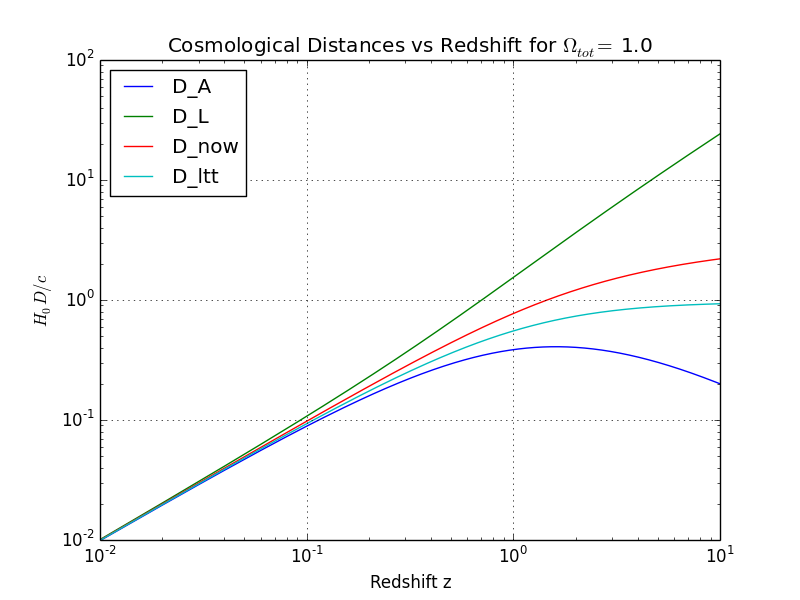
\includegraphics[width=0.6\textwidth]{cosmo_dist.png}
\caption{\footnotesize{\emph{Output from the cosmology calculator program, showing divergence between the different distance measures with increasing redshift. The dark blue line shows the angular diameter distance, the green line shows the luminosity distance, the red line shows the radial comoving distance and the light blue line the light travel distance.}}}
\label{fig:cosmo_calc}
\end{figure}    

\subsection{Analysing reduced SDSS spectra}\label{subsec:sdss_spec}
To motivate the development of a bespoke KMOS pipeline, we decided first to analyse the pre-reduced spectra of a set of normal, local SDSS galaxies. This back-to-front approach demonstrates the type of analysis that will be applied to KMOS galaxy spectra, albeit with significantly higher signal-to-noise than will be possible with the $z\sim 3$ KMOS galaxy sample. 
Broadly this section can be split into two categories, the first dealing with the extraction of emission line fluxes by fitting gaussians to the spectral locations of the emission lines. The second is the application of calibrated formulae to the parameters of the fitted gaussians to recover the physical properties of the galaxies. These categories are now discussed in turn.  

\subsubsection{Extracting Emission Line Fluxes}\label{subsub:ex_em}   
The reduced spectra were extracted from the `specObj' table of SDSS DR10 via SQL search. The SDSS database is a particularly useful testbed, as the optical emission line parameters as well as global galaxy properties derived from these are listed here and can be used for comparison.  The first stage of the analysis is to fit and subtract the continuum emission of the galaxy, here carried out in two separate ways. Either a third order polynomial is fit to the data, with emission lines masked, or a moving average is applied to match the continuum with a higher level of detail. Typically the simple polynomial fit provided emission line fluxes which matched the SDSS values more closely, and this is what is used throughout this section. Following continuum subtraction, it is necessary to know the redshift of the galaxy in order to determine the spectral locations of the emission line peaks. Here, and as would be the case in many other situations, the redshift of the galaxies is known and the wavelengths of the emission lines can be determined using the simple relation: 

\begin{equation}
\label{eq:redshift}
	\lambda _{peak} = (1 + z)\lambda _{vacuum}
\end{equation}

In the more general case where redshift is unknown, synthetic galaxy spectra can be used to give an indication of the expected shape of the galaxy SED. Early, intermediate and late-type synthetic spectra are plotted in Figure \ref{fig:temp_spec}. By shifting these synthetic spectra along a grid of redshift values and computing the cross correlation coefficient, $\rho$, with the observed spectrum after each shift, three separate $\rho$ arrays are determined. The maximum value of $\rho$ in each array corresponds to the redshift at which the observed and shifted template spectra best resemble each other. For these SDSS spectra, the late-type galaxy template produces by far the highest values of $\rho$ and the inferred galaxy redshift is always taken from this. An example of a cross correlation `power' plot against redshift for an observed spectrum and the shifted late-type template is shown in Figure \ref{fig:cross_cor}. The redshift value $z = 0.138$ agrees well with the value reported in the database.    \\ 




\begin{figure}[!htp]
\centering
\includegraphics[width=0.8\textwidth]{temp_spec.png}
\caption{\footnotesize{\emph{The synthetic spectra of early, intermediate and late-type galaxies, used for cross-correlation and redshift determination. Emission feautures becoming more prominent with age, as ionised nebulae become enriched by successive generations of star formation.}}}
\label{fig:temp_spec}
\end{figure} 

\begin{figure}[!htp]
\centering
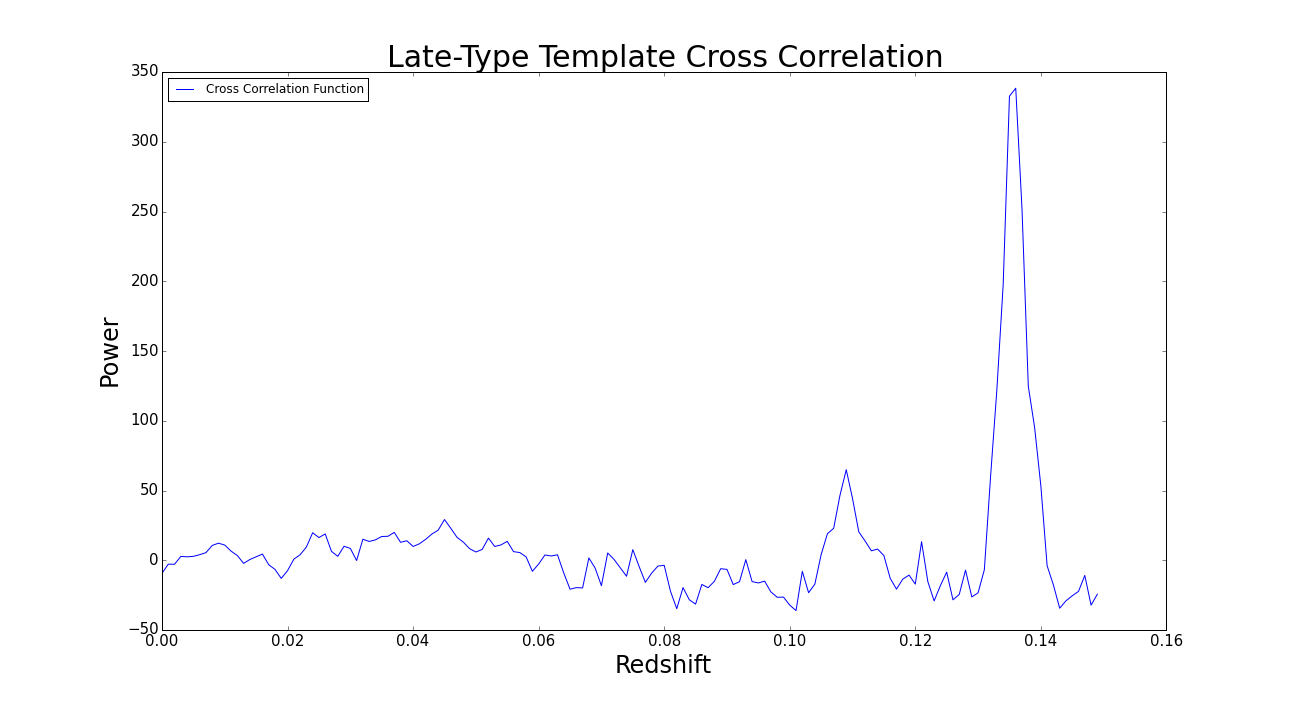
\includegraphics[width=0.8\textwidth]{Cross_corr.png}
\caption{\footnotesize{\emph{The cross correlation `power' is plotted against the grid of redshift values passed to the function, showing a clear peak at $z\sim 0.138$. This is a relatively easy procedure for such high quality spectra with prominent emission lines, becoming increasingly difficult to gain enough signal as redshift increases. }}}
\label{fig:cross_cor}
\end{figure} 

Once the redshift of the galaxy has been determined, equation \ref{eq:redshift} gives the recipe for finding the wavelengths of the peaks of the emission lines. A table of the known vacuum wavelengths for H$\beta$, [OIII]$\lambda 4959$, [OIII]$\lambda 5007$, H$\alpha$, [NII]$\lambda 6585$, [SII]$\lambda 6718$ and [SII]$\lambda 6732$ was used to find the observed wavelengths for each galaxy, and a gaussian function is fit to the data surrounding these emission line peaks in turn by fixing the central value. The area underneath the gaussian is the flux of that emission line and is also used to find the line equivalent width, whereas the width of the gaussian is used to determine the FWHM of the line, important for velocity measurements. A plot is made of the whole spectrum, with each emission line overlaid in red, to check the quality of these fits. Figure \ref{fig:fitted_spec} (a) gives an example of this, with panel (b) showing the wavelength region surrounding $H\alpha$ and confirming that the fitted gaussians closely match the shape of the emission lines.\\    

\begin{figure}[!htp]
\centering
\subfloat[]{\includegraphics[width=0.5\textwidth]{fitted_spectrum_full.png}}
\subfloat[]{\includegraphics[width=0.5\textwidth]{fitted_spectrum_part.png}}
\caption{\footnotesize{\emph{An example of one of the SDSS spectra for a $z\sim 0.14$ galaxy. Panel (a) shows the galaxy spectrum in blue, with the fitted gaussians overlaid in red. Panel (b) shows the same with an expanded view of the region $7400-7700\AA$, encompassing the $H\alpha$, $[NII]\lambda 6585$, $[SII]\lambda 6718$ and $[SII]\lambda 6732$ emission lines, shifted in wavelength by the factor $(1 + z)$. Plot (b) clearly demonstrates the high quality of the fit.}}}
\label{fig:fitted_spec}
\end{figure}



\subsubsection{Recovering Physical Properties}
After recovering line fluxes from the galaxy spectra, these can be converted to line luminosities using the luminosity distance, $D_{L}$, to the galaxy at redshift z computed with the cosmology calculator. For example, the luminosity of H$\alpha$ at redshift z, recovered from flux F($H\alpha$) is given by: 

\begin{equation}
\label{eq:flux-lum}
 	L(H\alpha) = 4\pi D_{L}^{2} F(H\alpha)
\end{equation} 

As mentioned in section \ref{subsubsec:em_lines}, H$\alpha$ is a particularly sensitive tracer of the instantaneous star formation rate, as only the most massive, and hence short lived, stars contribute significantly to the ionising photon flux. Using the relation provided in Kennicutt and Evans \citep{Kennicutt_2012}: 

\begin{equation}
 	\label{eq:halpha_sfr}
 	SFR(H\alpha) = log_{10}(L(H\alpha)) - 41.27
 \end{equation} 

an estimation of the SFR in each galaxy is be found. Also, using the PP04 \citep{Pettini_2004} and KD02 \citep{Kewley2002} abundance indicators (Equations \ref{eq:PP04} and \ref{eq:KD02} respectively), two separate estimations of the metal abundance are found. The PP04 indicator is found to agree relatively well with the SDSS oxygen abundance, but as described in \ref{subsec:abundance} there are discrepancies between the abundances reported from different indicators.  

\begin{equation}
	\label{eq:PP04}
	12 + log(O/H) = 9.12 + (0.73\frac{F([NII]\lambda 6585)}{F(H\alpha)})
\end{equation}

\begin{equation}
	\label{eq:KD02}
	12 + log(O/H) = 8.73 - (0.32\frac{F([OIII]\lambda 5007)F(H\alpha)}{F([NII]\lambda 6585)F(H\beta}))	
\end{equation}

As a final test of the accuracy of the emission line fluxes extracted from the SDSS spectra, a BPT diagram was plotted for a sample of 50,000 test galaxies in Figure \ref{fig:owen_bpt}. These data are a subset of the grey points in Figure \ref{fig:steidel_bpt} and the distributions closely resemble one another. The subset of galaxies with higher ionisation parameter are clearly seen as those with higher $\frac{[OIII]}{H\beta}$ for given $\frac{[NII]}{H\alpha}$.


\begin{figure}[!htp]
\centering
\includegraphics[width=0.7\textwidth]{bpt_owen.png}
\caption{\footnotesize{\emph{The BPT AGN diagnostic diagram recovered from applying the gaussian fitting procedure described above for a sample of 50,000 galaxies extracted from the specPhoto table of SDSS DR10. There is clear bimodality in the diagram, reflecting the ionisation state of galaxies with and without AGN.}}}
\label{fig:owen_bpt}
\end{figure}    

It would have been interesting to investigate stellar masses recovered from SPS modelling and recover the local MZ-relationship as well as the local SFR vs. $M_{*}$ curve, but we decided not to pursue stellar masses at this stage as this was more an introduction to the topic than a rigorous analysis. \\ 

It is likely that the  spectrum fitting strategy will have to be significantly aletered when moving to higher redshifts, fainter galaxies and lower S/N, but this was helpful for learning the general principles involved in extracting fluxes and galaxy physical properties from pre-reduced spectra. We finished this section towards the middle of December, turning attention to KMOS and the reduction pipeline at the end of December and after the Christmas break.   

\subsection{Additions to the KMOS reduction pipeline}\label{subsec:kmos_pipeline}

As described in section \ref{subsec:kmos_pipeline}, following the recipes supplied in the ESO reduction pipeline allows the user to process raw object images into fully reduced data cubes. However, the `out of the box' pipeline skips several steps which can greatly increase the quality of the reconstructed data cubes. The importance of these steps increases during the reduction of high redshift galaxy images, where the signal to noise ratio is significantly lower. It is important to tease as much information out from the data as possible at these redshifts, especially when measuring the strengths of nebular emission lines. Ground based near-IR spectroscopy is plagued by emission from the OH molecule, and so to extract reliable information from galaxy images, sky-subtraction must be performed as accurately as possible. The additions made to the ESO pipeline focus on improving the sky-subtraction process prior to science reconstruction, and correcting the infrared detectors for read noise effects. These additions are decsribed below.  \\ 
The overarching goal at this stage is to produce an automated pipeline which reliably extracts as much information as possible from the KMOS high redshift galaxy images. 

\subsubsection{Read noise}

The KMOS infrared detectors are read out in columns of 64 pixels, with a seperate amplifier for each column to boost the recorded signal. Each amplifier behaves differently to its neighbour, and the effect produced by one amplifier is not constant with time, leading to a banded flux bias effect across the sky subtracted object image, as shown in the top panel of Figure \ref{fig:column_sub}. This is carried through the data reduction pipeline, resulting in excess bands of flux across spatial pixels in the reconstructed object images. These problems reflect the current limitations of IR detectors and the difficulty of converting photon energies into electronic signals in this region of the spectrum. There are two different methods to compensate for this read bias, both involving a correction to the raw object image prior to sky subtraction. The image in Figure \ref{fig:column_sub} is ideal for testing this effect; the chosen detector is illuminated by the light from only 4 IFUs. This leaves a large `test-pixel section' not contaminated by sky/object flux in the centre of the detector for evaluating the quality of corrections made. The light blue curve in Figure \ref{fig:med_corr} shows the uniformity of spatial pixels prior to making any column-corretions, plotting the median of 100 spectral pixels for each spatial pixel in the test pixel section. Clearly the median jumps around, changing with each 64 or 128 pixel segment. \\ 

\begin{figure}[!htp]
\centering
\includegraphics[width=0.8\textwidth]{bad_column.png}
\includegraphics[width=0.8\textwidth]{good_column.png}
\caption{\footnotesize{\emph{The top panel shows a raw sky subtracted object image, whereas the bottom shows the same subtraction after the object image has been corrected for readout bias using the segments method. There is a significant improvement in the uniformity of the pixels after corretion. Both images show an 800x2048 section of one of the near-IR detectors, with 4 IFUs operational (these being the significantly brighter pixel columns).}}}
\label{fig:column_sub}
\end{figure}

The first correction method uses the top four spectral pixels of a raw sky subtracted object frame, these being masked `reference' pixels which are never illuminated by light from the IFUs. The correction is made by taking the median of these top four pixels in columns of 64, and subtracting this from each 64 pixel column of the object image prior to sky image subtraction. This accounts for pixel uniformity across the image, but still leaves the median value of the test pixel section offset from zero. The red curve of Figure \ref{fig:med_corr} shows the performance of this method, clearly improving the spatial uniformity of the uncorrected test pixel section.  \\ 

The second correction method uses the wavelength calibration `lcal' frame, output from the reduction pipeline. This frame has the same dimensions as the detector, contains `nan' values for pixels not illuminated by an IFU and the wavelength values of spectral pixels which are. There is a four pixel non-illuminated gap between each illuminated slitlet, and so by looking at pixels on the sky subtracted image corresponding to nan locations on the lcal frame, a column correction can be found.For each 64 pixel spatial column, the median value of the non-illuminated pixels of the subtracted image is found, and depending on whether this is negative or positive, it is either added or subtracted to the raw object image. A third correction method which uses a variation of this technique is also applied; instead of finding the correction in each 64x2048 column, the spectral axis is split into 128 pixel segments, and 16 64x128 corrections are found in each column. This caters for systematic variations in brightness across a detector not directly caused by readout bias. These two variations will be referred to as the lcal and lcal-segments correction methods. The dark blue and green curves of Figure \ref{fig:med_corr} respectively plot the performance of these two methods in the test pixel section. For the chosen frame the performance is equivalent, with the dark blue curve underneath the green, and the median pixel value shifted to zero. For further comparison between the raw and corrected sky subtracted frame, the counts per pixel in the test-pixel section were binned and a gaussian fit to the resultant histogram. The green and blue curves in Figure \ref{fig:pix_hist} show the pre and post-correction values respectively and demonstrate the shift of the median pixel value towards zero when the correction is applied.    \\       

Due to the lcal-segments method automatically shifting the median value of the test pixel segment to zero, this was chosen as the bias correction method for the pipeline. Since the bias effect varies between the detectors and the frames, the correction is applied in a script which passes the lcal-segments method all of the object-sky pairs in sequence. The correction is applied to each object frame, saving these with a `$\_$Corrected' extension.  


\begin{figure}[!htp]
\centering
\includegraphics[width=0.8\textwidth]{medians3.png}
\caption{\footnotesize{\emph{The performance of the three different column correction methods are compared against the median from the uncorrected sky subtracted object image. The light blue curve shows the uncorrected median, which jumps around in bands of 64 pixels, the red shows the top four method and both the dark blue and green curves lie on top of one another, demonstrating the lcal and lcal-segments methods respectively. The spatial uniformity of the pixels is greatly improved by all of the methods, and the two lcal methods also shift the median of the test pixel segment to zero.}}}
\label{fig:med_corr}
\end{figure}


\begin{figure}[!htp]
\centering
\includegraphics[width=0.6\textwidth]{pix_hist.png}
\caption{\footnotesize{\emph{To quantify the improvement made to the corrected subtracted image, a slice of pixels in between illuminated IFUs in both the raw and corrected subtracted images of Figure \ref{fig:column_sub} was extracted. The pixel values were placed in bins and a gaussian fit to the resultant histogram, blue for post-correction and green for pre-correction. The correction has the effect of shifting the median subtracted pixel value to zero, which is what we want for a clean sky subtraction. }}}
\label{fig:pix_hist}
\end{figure}





\subsubsection{OH Emission and Sky Subtraction}

Emission lines produced by the OH radical dominate near-IR spectra, appearing between 0.61 - 2.62 $\mu m$ and with fluxes several orders of magnitude larger than other sky emission. These are produced by Meinel rotation-vibration transitions of the OH molecule \citep{Meinel1950}, and appear in distinct bandings across the near-IR spectral range, as shown in Figure \ref{fig:sky_spec}. As a result, the removal of OH lines is an essential stage in the processing of near-IR data, with images of blank patches of sky being taken and then subtracted from the `object' images. Waves in the upper atmosphere cause a strong time dependence in both the absolute and relative intensities of these emission lines, complicating the removal process. For a clean subtraction, the flux of the OH lines in the sky and object images would have to vary by much less than 1 percent; yet the lines can vary significantly on time-scales of only a few minutes and often exposures times longer than this are required to achieve adequate S/N. To further complicate the subtraction process, manufacturing variations between instrument elements, and even small amounts of spectral flexure in the instrument during rotation can leave significant `P-Cygni' shaped residuals in the spectrum when a sky frame is subtracted. \\ 
So one cannot simply take the sky spectrum in one spatial pixel and subtract it from another, and for the reasons above, despite the rotation-vibration transitions of OH being very well understood \citep{Osterbrock1996}, attempts to generate and subtract synthetic OH spectra inevitably fail due to instrumental limitations and the time variation of OH emission. On a positive note, these lines serve as useful reference points for wavelength calibration of astronomical spectra, and near-IR sky emission line maps have been created to aid in the identification of these lines \citep{Rousselot2000}. Generally the flux variations of OH lines are not a problem for long-slit spectra, since the slit tends to be much more extended than the source. The OH lines can then be completely removed from the rectified two-dimensional spectrum by fitting a function to the background at each spectral pixel. For near-IR IFUs this cannot be done, since the field of view is much smaller and astronomical targets will occupy almost all of this, forcing the observation of separate blank sky fields.\\ 


\begin{figure}[!htp]
\centering
\includegraphics[width=0.8\textwidth]{sky_spectrum.png}
\caption{\footnotesize{\emph{A plot of the OH emission dominating the 1-1.4$\mu m$ region of the spectrum, extracted from a YJ-band KMOS skycube. The rotation-vibration bands of the OH molecule are clearly seen. These are extremely strong features, peaking at almost 5000 counts $s^{-1}$, orders of magnitude above the object flux.}}}
\label{fig:sky_spec}
\end{figure}

Davies \citep{Davies2007} describes a powerful method for subtracting these OH emission lines from reconstructed object datacubes. To a large extent, transitions between any two vibrational bands of the OH molecule lie between well defined wavelength limits. By splitting extracted spectra into these wavelength ranges and looking at the spectral pixels that contain bright OH lines in both the object and sky cubes, a wavelength dependent optimal scaling between the object and sky flux can be found. This is applied to the object cube to enable the best possible match between the amplitudes of the OH lines in object-sky pairs. A step by step guide to this procedure is given in the paper by Davies \citep{Davies2007}, and the essence of the algorithm is included optionally in the KMOS science reduction pipeline \footnote{To include optimal scaling of the skylines, the --skytweak=TRUE argument is supplied to the kmo\_sci\_red recipe.}. Applying the above scaling does not however account for the spectral shifts between object-sky pairs caused by the rotation of the instrument. There is an intermediate step in the Davies algorithm which shifts the object cube along the wavelength axis to best align OH lines. We question whether it is more appropriate to determine any spectral and spatial shifts from the raw images, prior to cube reconstruction. EXPLAIN WHY THIS WOULD BE BETTER. The following is a description of the algorithm I wrote to compute and apply these shifts to the raw images, before they are fed to the cube reconstruction recipes. \\ 

Panel (a) of Figure \ref{fig:column_sub} shows an example of a distinct set of P-Cygni features in a raw sky subtracted object image. These are the bandings of white and black horizontal lines which are clearly separated from one another, indicative of a misalignment between the raw object and sky images used for the subtraction. The goal is to find the optimal spatial ($\Delta x$) and spectral ($\Delta y$) pixel shifts which can be applied to the object frame to minimise this effect. The effect is said to be minimised when the correlation between the object and sky images is a maximum. This correlation is quantified by evaluating the cross-correlation coefficient, $\rho _{frames}$, between the object and sky frames using all `reliable' pixels on the 2D detector, given in Equation \ref{rho_frames}. $O_{xy}$, $S_{xy}$ are the individual object and sky pixels respectively, and $\overline{O}$, $\overline{S}$ are the mean values of the chosen pixels in the object and sky frames. 

\begin{figure}[!htp]
\centering
\subfloat[]{\includegraphics[width=0.32\textwidth]{pre_shift.png}}
\subfloat[]{\includegraphics[width=0.32\textwidth]{post_shift.png}}
\caption{\footnotesize{\emph{Panel (a) shows the distinct white/black pattern of the OH lines in the subtracted image before correcting the object. This effect would carry through to the extracted 1D spectrum, leaving a P-Cygni residual shape. Panel (b) shows the improvement made after applying the optimal shift. The subtraction leaves negative values in the place of the OH lines, which are then scaled up by the Davies skytweak algorithm.}}}
\label{fig:column_sub}
\end{figure}   

\begin{equation}
	\label{rho_frames}
	\rho_{frames} = \sum\limits_{x,y} \frac{(O_{xy} - \overline{O})(S_{xy} - \overline{S})}{\sqrt{(O_{xy} - \overline{O})^{2}(S_{xy} - \overline{S})^{2}}}
\end{equation}



Reliable pixels are those above a certain flux level indicative of real signal, those below an upper flux limit which would swamp the correlation coefficient and those which remain after masking the bad pixels returned by the KMOS calibration recipes for the same reason. In practice, we found that far better results are found when the bad pixel mask is `grown'. Although the recipes reveal the worst pixels, often the areas surrounding these are hot and contribute heavily to $\rho_{frames}$. Growing the mask refers to masking off an additional cross of pixels, one above, below, to the left and to the right, for every bad pixel identified in the calibrations. In short, the `reliable' pixels which remain are dominated by flux from the OH lines, which are exactly the structures we wish to correlate. The shift must be applied to the object due to the KMOS O-S-O observing strategy; each sky frame can be paired with two object frames and the shifts will be different each time. We expect that the shifts will be of order 0.1 pixels in both directions. Initially a grid of ($\Delta x$, $\Delta y$) pairs were constructed, ranging from $\Delta x, \Delta y = -0.5,-0.475,...0.5$ with 0.025 pixel increments and every value of $\Delta y$ explored for each $\Delta x$. Each pair is fed into the Pyraf `imshift' routine, which fits a function to the pixel surface and interpolates each new pixel value at the shift locations. $\rho _{frames}$ is computed for every shift, and the maximum value is chosen as indicator for the ($\Delta x, \Delta y$) pair to apply to each detector. Figure \ref{fig:column_sub} (b) shows the same column of pixels as in (a), with the optimal shift applied to the object prior to subtraction. There is a marked improvement over the original bandings, suggesting that the procedure has increased the alignment between object and sky frames. Figure \ref{fig:rho_plot} shows contours of the surface of $\rho _{frames}$ values computed over the grid passed to imshift. There is a clear, global maximum value at roughly ($\Delta x = 0.025, \Delta y = 0.055$) suggesting that the interpolant is well behaved. \\


       
\begin{figure}[!htp]
\centering
\includegraphics[width=0.7\textwidth]{KMOS_SPEC_OBS258_0009_Corrected110_temp_spline3_CorrelationGraph.png}
\caption{\footnotesize{\emph{A contour plot for $\rho$ computed for the grid of x, y shift values passed to Pyraf imshift. The contours are centred on the maximum value of $\rho$, this corresponding to the shift values which best align the object and sky images. The contours are drawn at $\rho _{max} - 0.25\sigma$, $\rho _{max} - 0.75\sigma$ and $\rho _{max} - 1.5\sigma$ and indicate the presence of a global maximum, suggesting unique `best' shift values $\Delta x$ and $\Delta y$.}}}
\label{fig:rho_plot}
\end{figure}

To check whether the recovered spectral shifts change as a function of position on each detector, the routine allows for each detector to be split into an arbitrary number of vertical and horizontal sections. The above process is then applied to each section in turn before recombining the shifted sections into the full detector. Generally we found that spatial variation in the shift is small, and that this starts to become a case of diminishing returns when the time required to apply the routine to all sections is taken into account. There are three detectors in every object frame, each accommodating eight IFUs, and in an observing block many frames will be collected to stack together. It is time consuming to pass the full grid of $(\Delta x, \Delta y)$ pairs to imshift, especially when segmenting each detector, and so to speed up the routine a downhill simplex algorithm is used. Values of $(\Delta x, \Delta y)$ which lead to increasing $\rho_{frame}$ evaluations are explored until a given precision is reached. This is a valid approach to take after verifying that there is a single $\rho_{frame}$ maximum, and greatly decreases the time taken to run the shift routine. In a similar way to the column correction method, the shift routine is applied to each object-sky pair in sequence, saving the shifted object with an extension indicating the number of horizontal and vertical segments each detector has been split into, e.g. ...\_11\_Shifted.fits. Figure \ref{fig:shift_plot} shows the values of ($\Delta x, \Delta y$) pairs for a series of frames, also plotted with instrument rotator angle to look for correlation. Clearly there is an oscillatory structure to the spectral shift, EXPLAIN OSCILLATORY STRUCTURE. \\ 


\begin{figure}[!htp]
\centering
\includegraphics[width=\textwidth]{shift_plot.png}
\caption{\footnotesize{\emph{The top panel shows the rotator angle, which shifts to its new value after every three detector ID's (single frame). The middle panel shows the disordered best shift $\Delta x$ values. The bottom panel shows the oscillatory structure recovered in the best $\Delta y$ values. This arises as a result of }}}
\label{fig:shift_plot}
\end{figure}

As an illustration of the improvement made by applying the shift, we examine the spectra of red-supergiant stars (extracted using the method described in section \ref{subsubsec:optimal_spec_extract}) from datacubes reconstructed in different ways. First, no shift is applied to the column corrected object frame before feeding through the reduction recipe, and the skytweak algorithm is not applied. The top panel of Figure \ref{fig:p_cygni} shows the spectrum extracted from one of the IFUs in the resultant datacube, plotted between 1.15-1.20$\mu m$ of the KMOS YJ-band, and with corresponding sky spectrum underneath. It is important to note the vastly different flux scales between the object and sky spectra, highlighting the importance of optimising the sky subtraction process. Clearly the spikes in the object spectrum correspond to the OH emission lines, and in this case show the P-Cygni profiles expected from applying no shift. Second, the shift routine is applied to the column corrected object frames and these are fed into the reduction recipe without skytweak applied. The middle panel of Figure \ref{fig:p_cygni} demonstrates the results of this, effectively eliminating the P-Cygni profile, but with the sky lines still in need of scaling. Third, the same is done as in the second analysis but with the skytweak option applied. The bottom panel of Figure \ref{fig:p_cygni} shows that the skylines are almost all successfully scaled away. This leaves the question of whether it is better to apply the shift to the raw data frames, or to the datacubes as part of the Davies algorithm. To test this, the column corrected object images were fed through the reduction pipeline with skytweak applied, allowing the algorithm to compute the spectral and spatial shifts from the skycube. A very similar plot to the bottom panel of Figure \ref{fig:p_cygni} is recovered, and a more detailed inspection is required to shed light on this question, a topic which is discussed in section \ref{frame_diagnostics}.


\begin{figure}[!htp]
\centering
\includegraphics[width=0.8\textwidth]{spec_compare_cygni.png}
\includegraphics[width=0.8\textwidth]{spec_compare.png}
\includegraphics[width=0.8\textwidth]{spec_compare_tweak.png}
\caption{\footnotesize{\emph{}}}
\label{fig:p_cygni}
\end{figure}

\subsubsection{Frame Diagnostics}\label{frame_diagnostics}
The quality of the sky subtraction can vary significantly on a frame by frame basis, and so when stacking many reconstructed datacubes to increase S/N for an object, one can carry through the results of poor sky subtractions to the whole stack. It is necessary to check the quality of sky subtraction on a frame by frame basis, by feeding a list of object/sky pairs through the science reconstruction recipe. The spectral locations of strong OH emission lines are found by examining a reconstructed skycube, and the quality of the sky subtraction is found for each IFU by taking a median of the stacked object flux at these wavelengths. Figure \ref{fig:sky_sub_perf} shows a summary of this diagnostic for the red-supergiant stars. The left panel shows the average sky subtraction performance across all IFUs for each science frame and the right panel plots for each frame the sky subtraction performance as a function of IFU. The most detailed view of the sky subtraction process is given in Figure \ref{fig:ifu_subplots}, which drills down to subplots of the sky subtraction performance in each IFU as a fuction of IFU frame. Note that the IFUs are arranged in rows of 8 to reflect the three detectors, and some of the IFUs were not operational during the exposures. There are two curves in Figure \ref{fig:ifu_subplots}; the blue curve represents the quality of the sky subtraction when the spectral shift is computed from the raw images using my algorithm; the red curve shows the quality when the shift is computed from the datacubes with the Davies algorithm. Clearly the performance is comparable, and sometimes the quality is better using each of the two methods. Currently, based solely upon an evaluation using YJ-band data, due to the raw frame shift being much more time intensive, the Davies algorithm is favourable. However, a more thorough analysis using data from the H and K-bands as well is required to properly understand the differences between the two methods. \\ 


From a combination of the plots in Figures \ref{fig:sky_sub_perf} and \ref{fig:ifu_subplots} it is easy to determine where the sky subtraction isn't performed as well, and hence which frames to omit from the stack. For example, in Figure \ref{fig:sky_sub_perf} frame 5 clearly has a far poorer sky subtraction than the rest. Omitting frame 5 from the stack significantly improves the quality of the extracted spectra. The reason for these spurious frames still isn't clear, and it is an ongoing process for us to understand why the sky subtraction process should sometimes be performed much worse than others. 


\begin{figure}[!htp]
\centering
\subfloat[]{\includegraphics[width=0.48\textwidth]{frame_performance.png}}
\subfloat[]{\includegraphics[width=0.48\textwidth]{IFU_by_frame.png}}
\caption{\footnotesize{\emph{The wavelengths of prominent OH emission lines are determined by looking at the spectrum of a skycube. A sky subtraction performance `statistic' is found by taking the median of the object cube flux at these wavelengths. The left panel shows the quality of the sky subtraction as a function of frame, taking an average of the statistic across all IFUs in the frame. The right panel shows the statistic as a function of IFU, plotted for each of the frames taken.}}}
\label{fig:sky_sub_perf}
\end{figure}

\begin{figure}[!htp]
\centering
\includegraphics[width=0.7\textwidth]{IFU_subplots_double.png}
\caption{\footnotesize{\emph{The sky subtraction performance is plotted in IFU as a function of frame. The blank plots are those IFUs which were not operational when the data were collected. This plot has the potential to highlight an optimal combination of frames to stack for each object. The blue curve represents the performance of the sky subtraction when the spectral shift is computed from the raw images and the red curve when the shift is computed from the datacubes with the Davies algorithm. It is difficult to distinguish in terms of performance a consistently `better' method, however the Davies algorithm is significantly faster to run.}}}
\label{fig:ifu_subplots}
\end{figure}

As a further frame-by-frame inspection, we check the PSF of a standard star for each of the frames. During an OB, KMOS dedicates one of the IFUs to observing a standard star, to monitor the variation in its PSF and hence variations in seeing as the night progresses. For the red-supergiants, a single bright object is chosen for this analysis. A 2D gaussian is fit to the object image and the FWHM of this gaussian gives an indication of the instantaneous seeing at the time the frame was observed. Figure \ref{fig:fwhm_track} shows the evolution of the FWHM of the standard star on the same night as the data in Figure \ref{fig:sky_sub_perf} were taken.

\begin{figure}[!htp]
\centering
\includegraphics[width=0.5\textwidth]{frame_fwhm.png}
\caption{\footnotesize{\emph{A standard star is tracked by one of the KMOS IFUs throughout the duration of the OB. This gives an indication of the seeing as each of the object frames are observed. The plot shows the evolution of the seeing throughout the course of the night, by tracking a bright star in one of the IFUs over all the frames, fitting a 2D gaussian to the flux, extracting the properties of the gaussian and converting to seeing using the pixel scale recorded in the fits header.}}}
\label{fig:fwhm_track}
\end{figure}

From the recovered FWHM of the 2D gaussian, the objects are divided into four bins of seeing quality. The `Best' bin has seeing better than 0.6$^{\prime\prime}$; the `Good' bin has seeing between 0.6$^{\prime\prime}$ and 1$^{\prime\prime}$. The `Okay' bin has seeing between 1$^{\prime\prime}$ and 1.5$^{\prime\prime}$; the `Bad' bin has anything worse than this, and typically any objects falling within this category are discarded. The objects in each of the four bins are then treated independently for optimal spectrum extraction as described in section \ref{subsubsec:optimal_spec_extract}. The motivation behind this procedure is that it would be unwise to degrade the quality of an image with good seeing, by stacking together in equal proportion with an object with bad seeing. The above analysis gives control over how stacking is carried out and which weights should be applied to the different seeing bins.  


\subsubsection{Optimal Integrated Spectrum Extraction}\label{subsubsec:optimal_spec_extract}

To increase S/N, it is necessary to extract the spectrum from a galaxy with weightings corresponding to where most of the flux is being emitted. Galaxies have a given radial profile, and light from each part of this profile is spread out into a seeing disc when it hits our atmosphere. Stars on the other hand are point-like, and the seeing disc from a star eminates from the same point-source of light. By tracking a star in one of the IFUs, we get a measure of the theoretical minimum seeing and can recover the set of weights which can be applied to each spatial pixel during the spectrum extraction. To expand on this, consider Figure \ref{fig:fwhm_image}. A 2D gaussian is fitted to the image of the tracked star in a particular object stack, recovering the parameters of the gaussian function. By normalising the gaussian to unity, and truncating the function at a given number of standard deviations from the centre, one recovers a weighting mask for spectrum extraction which can be applied to all objects in that stack by shifting the mask centre. The resultant 1D spectrum is then found by summing across all weighted spatial pixels. This procedure is applied to all of the FWHM bins described in the above section, to recover a set of `Best', `Good' and `Okay' 1D spectra for each of the objects observed by KMOS. In theory, an analysis similar to that described in section \ref{subsub:ex_em} is then applied to recover physical properties. 


\begin{figure}[!htp]
\centering
\includegraphics[width=0.7\textwidth]{gauss_img.png}
\caption{\footnotesize{\emph{An example of one of the 2D gaussian fits to the stacked `tracked' star in the `Best' FWHM bin. From this fit the profile for spectrum extraction is recovered.}}}
\label{fig:fwhm_image}
\end{figure}	


\subsubsection{Current Stage}
Automating the reduction pipeline as much as possible and applying to K and H-band, looking at getting galaxy raw data and extracting spatially resolved spectra.




\section{Planned projects}\label{sec:projects}
\subsection{The physical properties of galaxies at z = 3}
\subsubsection{Directly observing emission lines required for direct metallicity measurement}




\subsection{Searching for CIII $\&$ CIV Emission}
\citep{Zitrin2015}, \citep{Stark2015}



\subsection{Spectroscopic Confirmation of LAEs at z=7-8}

%%%%%%%%%%%%%%%%%%%%%%%%%%%%%%%%%%%%%%%%%%%%%%%%%%%%%%%%%%%%%%%%%%%%%%%%%%%%%%%%%%%%%%%%%%%%%%%%%%%%%%%%%%%%%%%%%%%%%%%%

\clearpage 
\bibliographystyle{apj.bst}
%\bibliography{/usr/local/texlive/texmf-local/bibtex/bib/ojt.bib}
\bibliography{/Users/owenturner/Documents/PhD/KMOS/Latex/Bibtex/library.bib}

\end{document}
